% Options for packages loaded elsewhere
% Options for packages loaded elsewhere
\PassOptionsToPackage{unicode}{hyperref}
\PassOptionsToPackage{hyphens}{url}
\PassOptionsToPackage{dvipsnames,svgnames,x11names}{xcolor}
%
\documentclass[
  letterpaper,
  DIV=11,
  numbers=noendperiod]{scrartcl}
\usepackage{xcolor}
\usepackage{amsmath,amssymb}
\setcounter{secnumdepth}{-\maxdimen} % remove section numbering
\usepackage{iftex}
\ifPDFTeX
  \usepackage[T1]{fontenc}
  \usepackage[utf8]{inputenc}
  \usepackage{textcomp} % provide euro and other symbols
\else % if luatex or xetex
  \usepackage{unicode-math} % this also loads fontspec
  \defaultfontfeatures{Scale=MatchLowercase}
  \defaultfontfeatures[\rmfamily]{Ligatures=TeX,Scale=1}
\fi
\usepackage{lmodern}
\ifPDFTeX\else
  % xetex/luatex font selection
\fi
% Use upquote if available, for straight quotes in verbatim environments
\IfFileExists{upquote.sty}{\usepackage{upquote}}{}
\IfFileExists{microtype.sty}{% use microtype if available
  \usepackage[]{microtype}
  \UseMicrotypeSet[protrusion]{basicmath} % disable protrusion for tt fonts
}{}
\makeatletter
\@ifundefined{KOMAClassName}{% if non-KOMA class
  \IfFileExists{parskip.sty}{%
    \usepackage{parskip}
  }{% else
    \setlength{\parindent}{0pt}
    \setlength{\parskip}{6pt plus 2pt minus 1pt}}
}{% if KOMA class
  \KOMAoptions{parskip=half}}
\makeatother
% Make \paragraph and \subparagraph free-standing
\makeatletter
\ifx\paragraph\undefined\else
  \let\oldparagraph\paragraph
  \renewcommand{\paragraph}{
    \@ifstar
      \xxxParagraphStar
      \xxxParagraphNoStar
  }
  \newcommand{\xxxParagraphStar}[1]{\oldparagraph*{#1}\mbox{}}
  \newcommand{\xxxParagraphNoStar}[1]{\oldparagraph{#1}\mbox{}}
\fi
\ifx\subparagraph\undefined\else
  \let\oldsubparagraph\subparagraph
  \renewcommand{\subparagraph}{
    \@ifstar
      \xxxSubParagraphStar
      \xxxSubParagraphNoStar
  }
  \newcommand{\xxxSubParagraphStar}[1]{\oldsubparagraph*{#1}\mbox{}}
  \newcommand{\xxxSubParagraphNoStar}[1]{\oldsubparagraph{#1}\mbox{}}
\fi
\makeatother


\usepackage{longtable,booktabs,array}
\usepackage{calc} % for calculating minipage widths
% Correct order of tables after \paragraph or \subparagraph
\usepackage{etoolbox}
\makeatletter
\patchcmd\longtable{\par}{\if@noskipsec\mbox{}\fi\par}{}{}
\makeatother
% Allow footnotes in longtable head/foot
\IfFileExists{footnotehyper.sty}{\usepackage{footnotehyper}}{\usepackage{footnote}}
\makesavenoteenv{longtable}
\usepackage{graphicx}
\makeatletter
\newsavebox\pandoc@box
\newcommand*\pandocbounded[1]{% scales image to fit in text height/width
  \sbox\pandoc@box{#1}%
  \Gscale@div\@tempa{\textheight}{\dimexpr\ht\pandoc@box+\dp\pandoc@box\relax}%
  \Gscale@div\@tempb{\linewidth}{\wd\pandoc@box}%
  \ifdim\@tempb\p@<\@tempa\p@\let\@tempa\@tempb\fi% select the smaller of both
  \ifdim\@tempa\p@<\p@\scalebox{\@tempa}{\usebox\pandoc@box}%
  \else\usebox{\pandoc@box}%
  \fi%
}
% Set default figure placement to htbp
\def\fps@figure{htbp}
\makeatother





\setlength{\emergencystretch}{3em} % prevent overfull lines

\providecommand{\tightlist}{%
  \setlength{\itemsep}{0pt}\setlength{\parskip}{0pt}}



 


\KOMAoption{captions}{tableheading}
\makeatletter
\@ifpackageloaded{caption}{}{\usepackage{caption}}
\AtBeginDocument{%
\ifdefined\contentsname
  \renewcommand*\contentsname{Table of contents}
\else
  \newcommand\contentsname{Table of contents}
\fi
\ifdefined\listfigurename
  \renewcommand*\listfigurename{List of Figures}
\else
  \newcommand\listfigurename{List of Figures}
\fi
\ifdefined\listtablename
  \renewcommand*\listtablename{List of Tables}
\else
  \newcommand\listtablename{List of Tables}
\fi
\ifdefined\figurename
  \renewcommand*\figurename{Figure}
\else
  \newcommand\figurename{Figure}
\fi
\ifdefined\tablename
  \renewcommand*\tablename{Table}
\else
  \newcommand\tablename{Table}
\fi
}
\@ifpackageloaded{float}{}{\usepackage{float}}
\floatstyle{ruled}
\@ifundefined{c@chapter}{\newfloat{codelisting}{h}{lop}}{\newfloat{codelisting}{h}{lop}[chapter]}
\floatname{codelisting}{Listing}
\newcommand*\listoflistings{\listof{codelisting}{List of Listings}}
\makeatother
\makeatletter
\makeatother
\makeatletter
\@ifpackageloaded{caption}{}{\usepackage{caption}}
\@ifpackageloaded{subcaption}{}{\usepackage{subcaption}}
\makeatother
\usepackage{bookmark}
\IfFileExists{xurl.sty}{\usepackage{xurl}}{} % add URL line breaks if available
\urlstyle{same}
\hypersetup{
  pdftitle={Como manter seu projeto organizado, seguro e acessível?},
  pdfauthor={ESTAT0090 -- Estatística Computacional  Prof.~Dr.~Sadraque E. F. Lucena  sadraquelucena@academico.ufs.br},
  colorlinks=true,
  linkcolor={blue},
  filecolor={Maroon},
  citecolor={Blue},
  urlcolor={Blue},
  pdfcreator={LaTeX via pandoc}}


\title{Como manter seu projeto organizado, seguro e acessível?}
\usepackage{etoolbox}
\makeatletter
\providecommand{\subtitle}[1]{% add subtitle to \maketitle
  \apptocmd{\@title}{\par {\large #1 \par}}{}{}
}
\makeatother
\subtitle{{Introdução ao RStudio + GitHub}}
\author{ESTAT0090 -- Estatística Computacional Prof.~Dr.~Sadraque E. F.
Lucena {sadraquelucena@academico.ufs.br}}
\date{}
\begin{document}
\maketitle


\subsection{Cenário profissional}\label{cenuxe1rio-profissional}

\subsubsection{Uma História Real (ou
quase)}\label{uma-histuxf3ria-real-ou-quase}

\begin{itemize}
\item
  Imagine que você é contratado por uma empresa para analisar dados de
  clientes e construir relatórios periódicos.
\item
  Você começa empolgado, faz seu código em R, roda tudo no seu
  computador e entrega um relatório lindo.
\item
  Um mês depois, o gerente pede que você refaça a análise com os novos
  dados.
\item
  Só tem um problema:

  \begin{itemize}
  \tightlist
  \item
    você não lembra qual script usou.
  \item
    Os arquivos estão todos em ``versão final\_v3\_final\_real.R''.
  \item
    E o relatório? Foi feito no Word e agora está com outro estagiário.
  \end{itemize}
\end{itemize}

\subsection{Cenário profissional}\label{cenuxe1rio-profissional-1}

\subsubsection{O Problema}\label{o-problema}

Você percebe que:

\begin{itemize}
\item
  Seus scripts estão bagunçados.
\item
  O histórico do que foi feito se perdeu.
\item
  O relatório não é reprodutível.
\item
  Ninguém (nem você mesmo) entende o que foi feito.
\end{itemize}

\subsubsection{A Motivação}\label{a-motivauxe7uxe3o}

Como resolver isso? Você precisa de:

\begin{itemize}
\item
  Um ambiente organizado para escrever e executar código (RStudio).
\item
  Um jeito de acompanhar o histórico do seu trabalho (Git).
\item
  Uma forma de colaborar e compartilhar com outras pessoas (GitHub).
\item
  Relatórios que podem ser reproduzidos a qualquer momento (Quarto).
\end{itemize}

\subsection{Um Exemplo da Nossa Própria
Disciplina}\label{um-exemplo-da-nossa-pruxf3pria-disciplina}

Cenário:

\begin{itemize}
\item
  Você está cursando Estatística Computacional.
\item
  A cada aula, o professor entrega:

  \begin{itemize}
  \item
    Slides da aula com explicações e um código em R.
  \item
    Um problema para você resolver, adaptando e expandindo o código.
  \end{itemize}
\item
  Você modifica, testa, ajusta e responde o problema.
\item
  Na aula seguinte, você parte exatamente de onde parou.
\end{itemize}

\subsection{\texorpdfstring{E se você fizer tudo isso com e
?}{E se você fizer tudo isso com  e ?}}\label{e-se-vocuxea-fizer-tudo-isso-com-e}

Você terá:

\begin{itemize}
\item
  Um histórico completo de aprendizagem.
\item
  Um repositório que mostra sua evolução.
\item
  Uma base reutilizável para projetos futuros.
\end{itemize}

\begin{quote}
É como criar seu próprio material interativo de Estatística
Computacional!
\end{quote}

\subsection{Objetivo da aula}\label{objetivo-da-aula}

\begin{itemize}
\tightlist
\item
  Entender o que é e para que serve o Git e o GitHub.
\item
  Saber como criar um repositório de projeto.
\item
  Atualizar repositório no GitHub via Studio.
\end{itemize}

\section{\texorpdfstring{Breve introdução ao
}{Breve introdução ao }}\label{breve-introduuxe7uxe3o-ao}

\subsection{O que é o ?}\label{o-que-uxe9-o}

\begin{itemize}
\item
  \textbf{Git} é uma ferramenta que \textbf{ajuda a controlar e
  gerenciar mudanças em arquivos} ao longo do tempo.
\item
  Ele permite que você \textbf{salve versões} diferentes de um trabalho
  à medida que faz alterações, de modo que possa \textbf{voltar para
  versões anteriores} se algo der errado ou se precisar revisar mudanças
  feitas.
\end{itemize}

\subsubsection{\texorpdfstring{Por que o é
importante?}{Por que o  é importante?}}\label{por-que-o-uxe9-importante}

\begin{itemize}
\item
  \textbf{Evita perda de trabalho:} Se você estiver escrevendo código ou
  criando qualquer tipo de documento, o Git permite que você
  \textbf{salve diferentes versões} do seu trabalho. Assim, se algo der
  errado, você pode voltar a uma versão anterior.
\item
  \textbf{Facilita o trabalho em equipe:} Quando várias pessoas estão
  trabalhando no mesmo projeto, o Git permite que cada uma
  \textbf{trabalhe de forma independente} e depois \textbf{una os
  trabalhos de maneira organizada}. Isso evita que as alterações de uma
  pessoa sobrescrevam as de outra.
\item
  \textbf{Organização e rastreamento:} O Git mantém um \textbf{histórico
  completo} de todas as mudanças feitas em um projeto, permitindo saber
  \textbf{quem fez o quê e quando}.
\end{itemize}

\subsection{O que é o ?}\label{o-que-uxe9-o-1}

\begin{itemize}
\item
  \textbf{GitHub} é uma plataforma online que \textbf{armazena e
  organiza projetos que utilizam Git}.
\item
  Ele permite que você \textbf{publique seu código, compartilhe arquivos
  e colabore com outras pessoas} em projetos de forma fácil e eficiente.
\end{itemize}

\subsubsection{\texorpdfstring{Por que o é
importante?}{Por que o  é importante?}}\label{por-que-o-uxe9-importante-1}

\begin{itemize}
\item
  \textbf{Armazenamento seguro:} Com o GitHub, seus projetos ficam
  \textbf{seguramente armazenados na nuvem}. Isso significa que você
  pode acessar seu trabalho de qualquer lugar e sempre terá uma cópia
  segura.
\item
  \textbf{Colaboração em equipe:} GitHub permite que várias pessoas
  trabalhem no mesmo projeto ao mesmo tempo. Cada pessoa pode fazer
  mudanças no código, e o GitHub ajuda a \textbf{gerenciar essas
  mudanças} sem que uma sobrescreva a outra.
\item
  \textbf{Histórico e transparência:} O GitHub mantém um
  \textbf{histórico completo} de todas as alterações feitas no seu
  projeto. Isso permite ver \textbf{quem fez o quê e quando},
  facilitando o acompanhamento e revisão do trabalho de equipe.
\end{itemize}

\subsection{\texorpdfstring{Como e por que usar o na
disciplina?}{Como e por que usar o  na disciplina?}}\label{como-e-por-que-usar-o-na-disciplina}

\begin{itemize}
\item
  Você receberá um script em R a cada aula
\item
  Durante a aula, vai editar esse script no RStudio, testando e
  resolvendo problemas
\item
  No final da aula, envia suas alterações para seu repositório (push)
  --- tudo salvo e organizado
\item
  Pode acessar seu trabalho de qualquer lugar, com segurança e histórico
  garantido
\end{itemize}

\begin{quote}
GitHub será seu \textbf{caderno digital de códigos} --- inteligente,
seguro e acessível para a disciplina
\end{quote}

\subsection{Primeiros passos}\label{primeiros-passos}

\begin{enumerate}
\def\labelenumi{\arabic{enumi}.}
\item
  Baixar e instalar o Git:
  \url{https://happygitwithr.com/install-git.html}
\item
  Criar uma conta no GitHub: \url{https://github.com/}
\item
  Criar um reposítório Git
\item
  Clone esse repositório para sua máquina usando o RStudio
\item
  Trabalhe no projeto e envie as atualizações de volta ao GitHub
\end{enumerate}

\begin{quote}
Desenvolva o hábito de buscar soluções por conta própria. Isso faz parte
do dia a dia de quem trabalha com dados. Comece agora a desenvolver essa
autonomia.
\end{quote}

\subsection{\texorpdfstring{Criando um repositório no
}{Criando um repositório  no }}\label{criando-um-reposituxf3rio-no}

\begin{itemize}
\item
  Após fazer login no GitHub, Clique em \texttt{+} no canto superior
  direito
\item
  Em seguida, clique em \texttt{New\ repository}
\end{itemize}

\subsection{\texorpdfstring{Criando um repositório no
}{Criando um repositório  no }}\label{criando-um-reposituxf3rio-no-1}

\begin{itemize}
\item
  Em \texttt{Repository\ name} dê um anome ao repositóro
\item
  Em \texttt{Description} faça uma descrição do repositório
\item
  Marque a opção \texttt{Public} ou \texttt{Private}
\item
  Em \texttt{Initialize\ this\ repository\ with:} marque a opção
  \texttt{Add\ a\ README\ file}
\item
  Clique em \texttt{Create\ repository}
\end{itemize}

\begin{center}
\pandocbounded{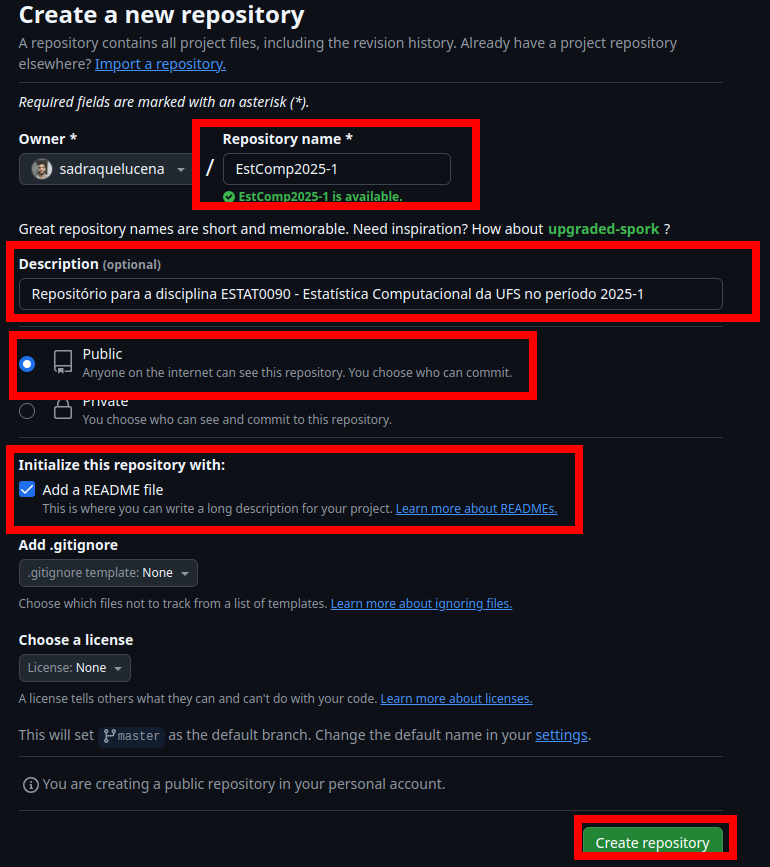
\includegraphics[keepaspectratio]{imagens/github2.png}}
\end{center}

\subsection{}\label{section}

\begin{itemize}
\item
  Com o repositório já criado no GitHub, agora vamos usar o RStudio para
  \textbf{ligar o projeto local ao repositório remoto}.
\item
  Assim, todas as alterações feitas no RStudio poderão ser
  \textbf{salvas na nuvem} e \textbf{versionadas automaticamente}.
\item
  Para enviar essas alterações ao GitHub, será necessário se autenticar
  --- com \textbf{login e senha} ou com um \textbf{token de acesso}.

  \begin{itemize}
  \tightlist
  \item
    Vamos ver como criar um token de acesso no GitHub.
  \end{itemize}
\end{itemize}

\subsection{\texorpdfstring{Criando um token de acesso no
}{Criando um token de acesso no }}\label{criando-um-token-de-acesso-no}

\begin{enumerate}
\def\labelenumi{\arabic{enumi}.}
\tightlist
\item
  Estando logado no GitHub, clique na sua \textbf{foto de perfil} no
  canto superior direito\\
\item
  Clique em \texttt{Settings}
\end{enumerate}

\subsection{\texorpdfstring{Criando um token de acesso no
}{Criando um token de acesso no }}\label{criando-um-token-de-acesso-no-1}

\begin{enumerate}
\def\labelenumi{\arabic{enumi}.}
\setcounter{enumi}{2}
\tightlist
\item
  No canto inferior esquerdo da tela clique em
  \texttt{Developer\ settings}
\end{enumerate}

\subsection{\texorpdfstring{Criando um token de acesso no
}{Criando um token de acesso no }}\label{criando-um-token-de-acesso-no-2}

\begin{enumerate}
\def\labelenumi{\arabic{enumi}.}
\setcounter{enumi}{3}
\item
  No canto superior esquerdo da tela clique em
  \texttt{Personal\ access\ tokens}
\item
  Clique em \texttt{Tokens\ (classic)}
\end{enumerate}

\begin{enumerate}
\def\labelenumi{\arabic{enumi}.}
\setcounter{enumi}{5}
\item
  Em \texttt{Expiration} selecione a data em que o token irá expirar
\item
  Marque todas as opções em \texttt{Select\ scopes}
\item
  Clique em \texttt{Generate\ token}
\end{enumerate}

\begin{quote}
O token será gerado uma única vez. Guarde-o com cuidado, pois não será
possível visualizá-lo novamente no GitHub. Você usará esse token quando
for solicitada autenticação.
\end{quote}

\section{\texorpdfstring{Integrando e
}{Integrando  e }}\label{integrando-e}

\subsection{\texorpdfstring{ + : integração
prática}{ + : integração prática}}\label{integrauxe7uxe3o-pruxe1tica}

\begin{itemize}
\item
  O \textbf{RStudio} possui integração nativa com o \textbf{Git} e
  \textbf{GitHub}

  \begin{itemize}
  \item
    Ou seja, é possível sincronizar um repositório GitHub a um
    repositório local
  \item
    Isso significa que você pode ligar o repositório do GitHub (na
    nuvem) ao seu projeto no computador. Assim, o que você altera
    localmente pode ser enviado para o GitHub --- e vice-versa.
  \end{itemize}
\item
  Para isso, seguimos os seguintes passos:
\end{itemize}

\begin{enumerate}
\def\labelenumi{\arabic{enumi}.}
\item
  Fazemos uma cópia do repositório do GitHub na máquina local usando o
  RStudio.

  \begin{itemize}
  \tightlist
  \item
    Quando já há uma cópia na máquina, começamos o trabalho atualizando
    o projeto local com as alterações que estão no GitHub
    (\texttt{pull}).
  \end{itemize}
\item
  Trabalhamos normalmente no projeto: scripts, análises,
  relatórios\ldots{}
\item
  Usamos o Git para \textbf{registrar as alterações} (\texttt{commit}) e
  \textbf{enviar para o GitHub} (\texttt{push}).
\end{enumerate}

\subsection{\texorpdfstring{ + : criando o projeto
local}{ + : criando o projeto local}}\label{criando-o-projeto-local}

\begin{itemize}
\tightlist
\item
  No canto superior direito do RStudio clique em
  \texttt{File\ \textgreater{}\ New\ Project}
\end{itemize}

\begin{itemize}
\tightlist
\item
  Clique em \texttt{Version\ control}
\end{itemize}

\subsection{\texorpdfstring{ + : criando o projeto
local}{ + : criando o projeto local}}\label{criando-o-projeto-local-1}

\begin{itemize}
\tightlist
\item
  Clique em \texttt{Git}
\end{itemize}

\subsection{\texorpdfstring{ + : criando o projeto
local}{ + : criando o projeto local}}\label{criando-o-projeto-local-2}

\begin{itemize}
\item
  No campo \texttt{Repository\ URL}, cole a URL do repositório que você
  criou no GitHub
\item
  Em \texttt{Create\ project\ as\ subdirectory\ of}, escolha o diretório
  em que o repositório do GitHub será copiado na máquina local
\item
  Clique em \texttt{Create\ Project}
\end{itemize}

\subsection{\texorpdfstring{ + : criando o projeto
local}{ + : criando o projeto local}}\label{criando-o-projeto-local-3}

\begin{itemize}
\item
  Se você estiver clonando um \textbf{repositório público}, o RStudio
  irá criar uma cópia do projeto localmente, sem exigir login.
\item
  Se o repositório for \textbf{privado}, o GitHub pedirá que você se
  autentique (login e senha ou token).
\end{itemize}

\section{\texorpdfstring{Atualizando repositório no
}{Atualizando repositório no }}\label{atualizando-reposituxf3rio-no}

\subsection{\texorpdfstring{Enviando alterações para o via
}{Enviando alterações para o  via }}\label{enviando-alterauxe7uxf5es-para-o-via}

\begin{itemize}
\item
  Depois de salvar as atualizações do seu projeto local, você pode
  \textbf{enviar essas alterações para o repositório no GitHub
  diretamente pelo RStudio}.
\item
  Você deve fazer:
\end{itemize}

\begin{enumerate}
\def\labelenumi{\arabic{enumi}.}
\tightlist
\item
  No quadrante superior direito clique em \texttt{Commit}
\end{enumerate}

\subsection{\texorpdfstring{Enviando alterações para o via
}{Enviando alterações para o  via }}\label{enviando-alterauxe7uxf5es-para-o-via-1}

\begin{enumerate}
\def\labelenumi{\arabic{enumi}.}
\setcounter{enumi}{1}
\item
  RStudio mostra os arquivos que foram alterados. Selecione-os
\item
  No campo \texttt{Commit\ message} escreva um comentário contendo o que
  foi atualizado
\item
  Clique em \texttt{Commit}
\end{enumerate}

\subsection{\texorpdfstring{Enviando alterações para o via
}{Enviando alterações para o  via }}\label{enviando-alterauxe7uxf5es-para-o-via-2}

\begin{enumerate}
\def\labelenumi{\arabic{enumi}.}
\setcounter{enumi}{4}
\tightlist
\item
  Clique em \texttt{Close}
\end{enumerate}

\subsection{\texorpdfstring{Enviando alterações para o via
}{Enviando alterações para o  via }}\label{enviando-alterauxe7uxf5es-para-o-via-3}

\begin{enumerate}
\def\labelenumi{\arabic{enumi}.}
\setcounter{enumi}{5}
\item
  Note que irá aparecer a mensagem
  \texttt{Your\ branch\ is\ ahead\ of\ \textquotesingle{}origin/master\textquotesingle{}\ by\ 1\ commit}
\item
  Clique em \texttt{Push}
\end{enumerate}

\begin{enumerate}
\def\labelenumi{\arabic{enumi}.}
\setcounter{enumi}{7}
\tightlist
\item
  No campo
  \texttt{Username\ for\ \textquotesingle{}https://github.com\textquotesingle{}}
  coloque login e clique em \texttt{OK}
\end{enumerate}

\subsection{\texorpdfstring{Enviando alterações para o via
}{Enviando alterações para o  via }}\label{enviando-alterauxe7uxf5es-para-o-via-4}

\begin{enumerate}
\def\labelenumi{\arabic{enumi}.}
\setcounter{enumi}{8}
\item
  No campo \texttt{Personal\ Access\ Token} insira o token criado no
  GitHub
\item
  Clique em \texttt{OK}
\end{enumerate}

\subsection{\texorpdfstring{Enviando alterações para o via
}{Enviando alterações para o  via }}\label{enviando-alterauxe7uxf5es-para-o-via-5}

\begin{enumerate}
\def\labelenumi{\arabic{enumi}.}
\setcounter{enumi}{10}
\tightlist
\item
  Caso apareça a mensagem abaixo, os arquivos foram atualizados no
  repositório do GitHub.
\end{enumerate}

\subsection{Material Extra}\label{material-extra}

Aprofunde o que vimos em aula com esses vídeos no YouTube:

\begin{itemize}
\item
  Curso completo de Git e GitHub: \textless http://tiny.cc/GitGitHub:
\item
  Integração do RStudio com o GitHub:

  \begin{itemize}
  \tightlist
  \item
    Parte 1: \url{http://tiny.cc/RStudioGitHub1}
  \item
    Parte 2: \url{http://tiny.cc/RStudioGitHub2}
  \end{itemize}
\end{itemize}

\subsection{Ganhos da aula}\label{ganhos-da-aula}

\begin{itemize}
\item
  Versionamento de cpodigo e arquivos com GitHub
\item
  Integração do RStudio com GitHub
\item
  Experiência com ferramentas do mercado
\end{itemize}

\subsection{Atividade extraclasse}\label{atividade-extraclasse}

\subsubsection{Configure seu ambiente de trabalho
pessoal}\label{configure-seu-ambiente-de-trabalho-pessoal}

\paragraph{Objetivo}\label{objetivo}

Deixar seu computador pessoal pronto para continuar os trabalhos da
disciplina fora do laboratório, de forma independente.

\paragraph{Etapas:}\label{etapas}

\begin{itemize}
\item
  Instalar o Git: \url{https://happygitwithr.com/install-git.html}
\item
  Instalar o R: \url{https://cran.r-project.org}
\item
  Instalar o RStudio: \url{https://posit.co/download/rstudio-desktop}
\item
  Fazer uma cópia (clone) do \textbf{repositório da disciplina no
  GitHub} para o seu computador.
\end{itemize}

Criar um \textbf{repositório de teste}, clonar no RStudio e fazer seu
\textbf{primeiro commit}.

\section{Fim}\label{fim}




\end{document}
